\section{Auswertung}
\label{sec:Auswertung}


\subsection{Statische Methode}
In den folgenden Plots werden jeweils zwei Temperaturverläufe verglichen. In Abbildung \ref{fig:t1t4} wird der breite und der schmale 
Messingstab untersucht, in Plot\ref{fig:t5t8} werden Aluminium und Edelstahl auf ihre Temperaturen untersucht. Die Temperaturen werden hier jeweils
an den vom Thermoelement weiter entfernten Thermometern gemessen.

\begin{figure}[H]
    \centering
    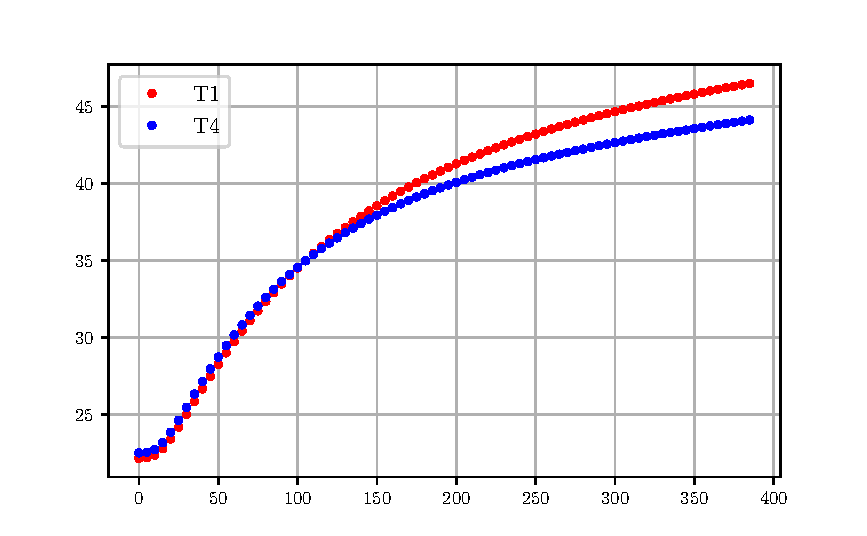
\includegraphics[width=\textwidth]{build/T1T4.pdf}
    \caption{Temperaturverläufe der Messingstäbe.}
    \label{fig:t1t4}
\end{figure}

\begin{figure}[H]
    \centering
    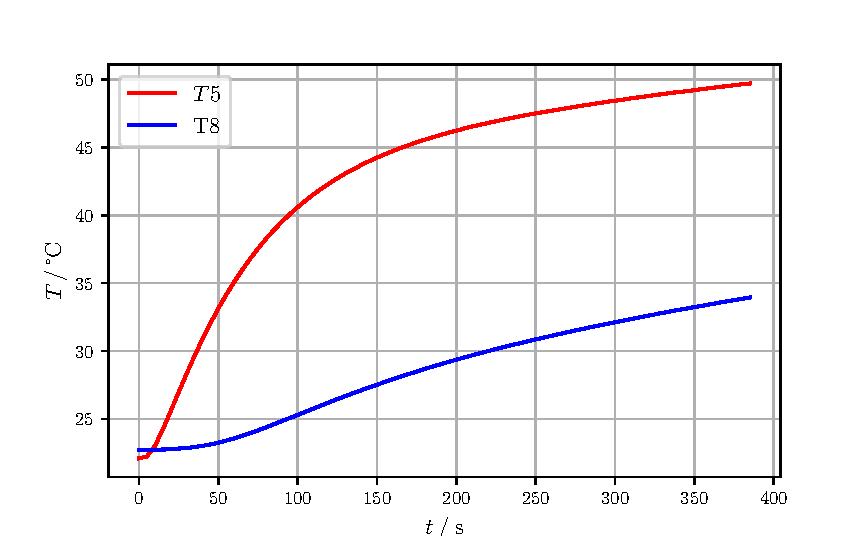
\includegraphics[width=\textwidth]{build/T5T8.pdf}
    \caption{Temperaturverläufe von Aluminium und Edelstahl.}
    \label{fig:t5t8}
\end{figure}

In der Auflistung stehen die in den Plots gezeigten Temperaturen zu Ende der statischen Messung:
\begin{align*}
T_1(t=385) =& 46.50 \si{\celsius}\\
T_4(t=385) =& 44.13 \si{\celsius}\\
T_5(t=385) =& 49.71 \si{\celsius}\\
T_8(t=385) =& 33.94 \si{\celsius}
\end{align*}

%Es ist zu sehen, dass die Temperatur des Aluminiumstabes am höchsten ist. Da alle Thermometer den gleichen Abstand
%zum Heizkörper haben und deren anfängliche Temperaturen bis auf geringe Abweichungen gleich sind, kann daraus 
%geschlossen werden, dass Aluminium die höchste Wärmeleitfähigkeit hat.

Zur Berechnung des Wärmestroms wird die Querschnittsfläche $A$ der einzelnen Stäbe aus der Versuchsanleitung entnommen.
Die Wärmeleitfähigkeiten $\kappa$ sind aus der Literatur\cite{V204} übernommen und die Entfernung $\Delta x$ der jeweiligen $T$ 
werden abgemessen.

\begin{align*}
\kappa _\text{Messing}& = 109\si{\watt\per\meter\kelvin} \\
A_\text{Messing,breit}& = 48\cdot 10^{-6}\si{\meter\squared} \\
\Delta x_\text{Messing,breit}& = 0,03\si{\meter} \\
\kappa _\text{Edelstahl}& = 16\si{\watt\per\meter\kelvin} \\
A_\text{Edelstahl}& = 48\cdot 10^{-6}\si{\meter\squared} \\
\Delta x_\text{Edelstahl}& = 0,03\si{\meter} \\
\kappa_\text{Aluminium}& = 205 \si{\watt\per\meter\kelvin}
\end{align*}

\begin{table}[H]
    \centering
    \caption{Wäremestrom von Messing und Edelstahl.}
    \label{tab:deltaq}
    \begin{tabular}{S S S S S}
        \toprule
        {$t\:/\:\si{s}$} & {$\Delta T_{21}\:/\:\si{\kelvin}$} & {$\frac{\text{d}Q_{21}}{\text{d}t}\:/\:\si{\watt}$} & 
        {$\Delta T_{78}\:/\:\si{\kelvin}$} & {$\frac{\text{d}Q_{78}}{\text{d}t}\:/\:\si{\watt}$} \\
        \midrule
        75 & 7.11 & 1.23998 & 12.65 & 0.32384 \\
        150 & 4.80 & 0.83712 & 13.52 & 0.34611 \\
        225 & 3.55 & 0.61912 & 12.57 & 0.32179 \\
        300 & 2.93 & 0.51099 & 11.77 & 0.30131 \\
        375 & 2.61 & 0.45518 & 11.21 & 0.28698 \\
        \bottomrule 
    \end{tabular}
\end{table}
Der folgende Plot vergleicht die Temperaturunterschiede der nahen und fernen Thermometer des jeweils gleichen Stabs. Dieser 
Temperaturunterschied ist hier für Messing und Edelstahl gezeigt.

\begin{figure}[H]
    \centering
    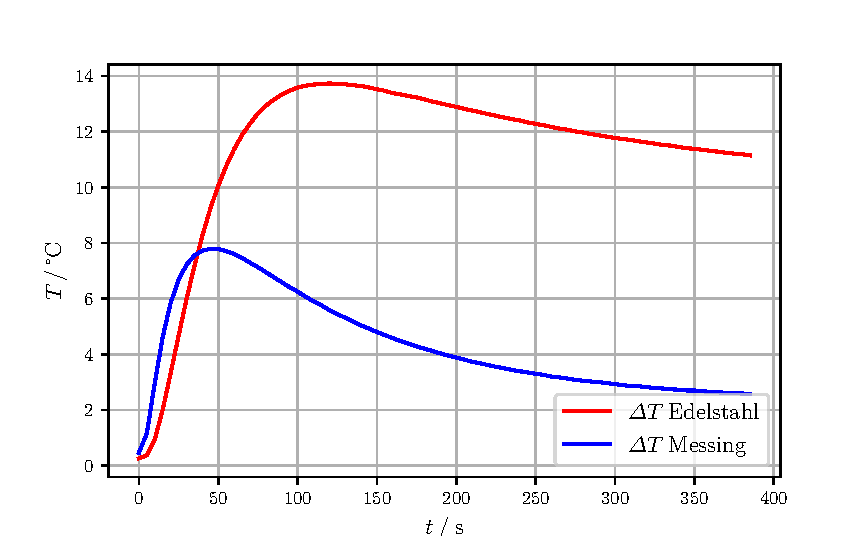
\includegraphics[width=\textwidth]{build/deltaT.pdf}
    \caption{Temperaturunterschied innerhalb eines Stabes für Messing und Edelstahl.}
    \label{fig:deltat}
\end{figure}


\subsection{Dynamische Methode}

Im Folgenden wird anhand der Temperaturamplituden $A_i$ und der Phasendifferenzen $\Delta t$ die Wärmeleitfähigkeit $\kappa$
der verschiedenen Metalle berechnet. Für Messing und Aluminium wird dafür die Messung mit 80$\si{\s}$ Periodendauer 
und für Edelstahl die Messung mit 200$\si{\s}$ Periodendauer verwendet.
Die Amplituden, sowie die Phasendifferenzen können aus den Messwerten abgelesen werden. Dabei wird jeweils die Differenz zwischen einem Maximum und dem 
Mittel der umgebenden Minima gebildet. Der so erechnete Wert wird im Folgenden als Amplitude angegeben.
 Damit kann nach Gleichung\ref{eqn:kappa}
jeweils $\kappa$ berechnet werden.

\begin{table}[H]
    \centering
    \caption{Amplituden und Phasendifferenz der Temperaturverläufe von Messing.}
    \label{tab:amp_m}
    \begin{tabular}{S S S}
        \toprule
        {$A_1\:/\:\si{\kelvin}$} & {$A_2\:/\:\si{\kelvin}$} & {$\Delta t\:/\:\si{\s}$} \\
        \midrule
        4.585 & 12.890 & 16 \\
        4.245 & 12.705 & 14 \\
        4.070 & 12.555 & 13 \\
        \bottomrule
    \end{tabular}
\end{table}

\begin{figure}[H]
    \centering
    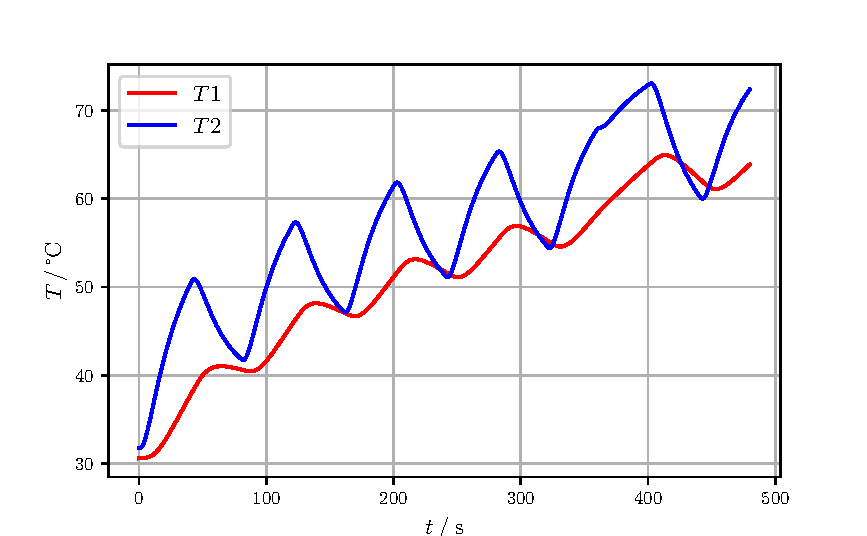
\includegraphics[width=\textwidth]{build/T1T2.pdf}
    \caption{Temperaturunterschied innerhalb des Messingstabes.}
    \label{fig:t1t2}
\end{figure}

Die Konstanten für Messing sind:
\begin{align*}
    \rho& = 8520\:\si{\kilo\gram\per\meter\cubed} \\
    c& = 385\:\si{\joule\per\kilo\gram\kelvin}
\end{align*}

Daraus ergibt sich mit der Gleichung\ref{eqn:kappa} für die Wärmeleitfähigkeit:
\begin{equation*}
    \kappa_{\text{Messing}} = \SI{95(7)}{\watt\per\meter\kelvin}
\end{equation*}   

\begin{table}[H]
    \centering
    \caption{Amplituden und Phasendifferenz der Temperaturverläufe von Aluminium.}
    \label{tab:amp_a}
    \begin{tabular}{S S S}
        \toprule
        {$A_5\:/\:\si{\kelvin}$} & {$A_6\:/\:\si{\kelvin}$} & {$\Delta t\:/\:\si{\s}$} \\
        \midrule
        8.060 & 15.955 & 8 \\
        7.635 & 15.600 & 7 \\
        7.500 & 15.515 & 7 \\
        \bottomrule
    \end{tabular}
\end{table}

\begin{figure}[H]
    \centering
    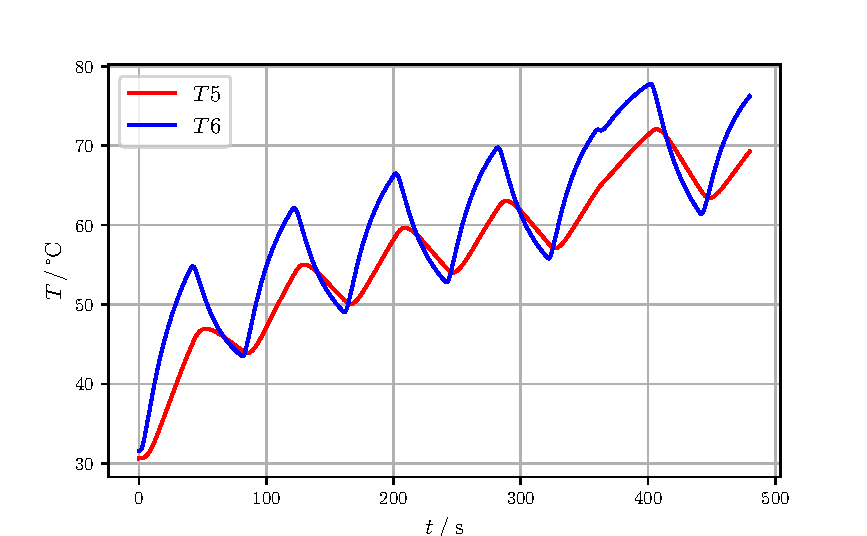
\includegraphics[width=\textwidth]{build/T5T6.pdf}
    \caption{Temperaturunterschied innerhalb des Aluminiumstabes.}
    \label{fig:t5t6}
\end{figure}

Die Konstanten für Aluminium sind:
\begin{align*}
    \rho& = 2800\:\si{\kilo\gram\per\meter\cubed} \\
    c& = 850\:\si{\joule\per\kilo\gram\kelvin}
\end{align*}

Daraus ergibt sich für die Wärmeleitfähigkeit:
\begin{equation*}
    \kappa_{\text{Aluminium}} = \SI{202(11)}{\watt\per\meter\kelvin}
\end{equation*}

\begin{table}[H]
    \centering
    \caption{Amplituden und Phasendifferenz der Temperaturverläufe von Edelstahl.}
    \label{tab:amp_e}
    \begin{tabular}{S S S }
        \toprule
        {$A_7\:/\:\si{\kelvin}$} & {$A_8\:/\:\si{\kelvin}$} & {$\Delta t\:/\:\si{\s}$} \\
        \midrule
        19.575 & 3.110 & 66 \\
        19.410 & 2.920 & 60 \\
        19.515 & 2.955 & 46 \\
        19.040 & 2.610 & 51 \\
        \bottomrule
    \end{tabular}
\end{table}

\begin{figure}[H]
    \centering
    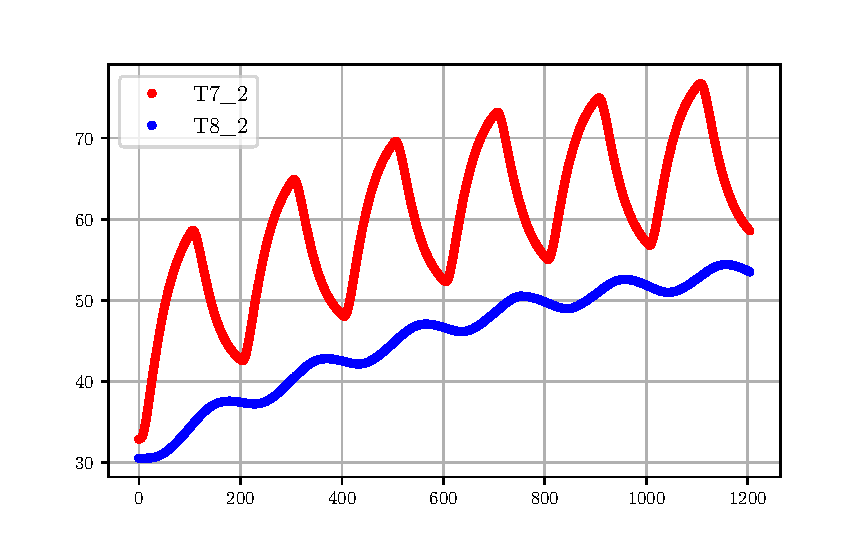
\includegraphics[width=\textwidth]{build/T7T8.pdf}
    \caption{Temperaturunterschied innerhalb des Edelstahlstabes.}
    \label{fig:t7t8}
\end{figure}

Die konstanten für Edelstahl sind:
\begin{align*}
    \rho& = 8000\:\si{\kilo\gram\per\meter\cubed} \\
    c& = 400\:\si{\joule\per\kilo\gram\kelvin}
\end{align*}

Daraus ergibt sich für die Wärmeleitfähigkeit:
\begin{equation*}
    \kappa = \SI{13.6(11)}{\watt\per\meter\kelvin}
\end{equation*}
